\documentclass[a4paper,12pt,twoside]{report}
\usepackage{rotating}
\usepackage{float}

\usepackage[english,french]{babel}
\usepackage[utf8]{inputenc}
\usepackage[T1]{fontenc}
\usepackage{fancyhdr}
\usepackage{graphicx}
\usepackage[outerbars]{changebar}
\usepackage{caption}
\usepackage{xcolor}
\usepackage{url}
\usepackage{multicol}
\usepackage{enumitem}

\usepackage{makeidx}
\usepackage[colorlinks]{hyperref}
\usepackage[acronym]{glossaries}
\usepackage{geometry}
\usepackage[titletoc]{appendix}

%\selectlanguage{francais}

\makeglossaries
\makeindex

\geometry{vmargin=3cm}
\hypersetup{%
  citecolor=black
}
%\newacronym[\glsshortpluralkey=cas,\glslongpluralkey=contrived
%acronyms]{aca}{aca}{a contrived acronym}
%
%\newglossaryentry{sample}{name={sample},description={a sample entry}}
%
%\addto\captionsfrench{
%\renewcommand{\acronymname}{Acronymes}%
%}
%
%\addto\captionsfrench{
%\renewcommand{\glossarymname}{Glossaire}%
%}

\setcounter{secnumdepth}{3}

\fancyhf{}
\fancyhead[LE]{\slshape \rightmark} %section
\fancyhead[RE]{\thepage}
\fancyhead[RO]{\slshape \leftmark} % chapter
\fancyhead[LO]{\thepage}
\pagestyle{fancy}

\lfoot{\tiny\textsl{IDSCC5 - ENSAO}}

\cfoot{\tiny\textsl{Academic Year 2022 - 2023}}

\rfoot{\tiny\textsl{Rapport PFE}}

\addto\captionsfrench{
\renewcommand{\listfigurename}{List of Figures}%
}

\begin{document}

\begin{titlepage}

\fontfamily{cmr}\selectfont

\begin{center}
    
\includegraphics[scale=0.1]{images/ump}\hfill
    \LARGE Université Mohammed Premier\hfill
    
\includegraphics[scale=0.1]{images/ump}\par
    \Large Ecole Nationale des Sciences Appliquées\par
    \Large Oujda\vfill
    \Large\textbf{End of Studies Project Report}\par
    \large Data Science \& Cloud Computing\par
    \textit{\textbf{Defended on:} 21/07/2023}\par
\end{center}



\begin{center}
    \hrulefill\par
    \LARGE Designing, Developing, and Deploying Innovative Solutions using Artificial Intelligence and Natural Language Processing in a Multidisciplinary Context\par
    \hrulefill\par
\end{center}
\vfill

\begin{center}
\textbf{By:}
    MEHDI Ibrahim

\end{center}

\vfill


\begin{multicols}{2}
\noindent \textbf{Jury Members:}
\begin{itemize}[label=\textbullet, leftmargin=*]
  \item \textbf{Prof.} KOULALI Mohamed Amine
  % Add more jury members as needed
\end{itemize}

\columnbreak

\noindent \textbf{Supervisors:}
\begin{itemize}[label=\textbullet, leftmargin=*]
  \item \textbf{Prof.} KOULALI Mohamed Amine
  \item \textbf{Dr.} PERFETTO Anna
  \item \textbf{M.} MIRON Jean-Raphaël
  % Add more supervisors as needed
\end{itemize}

\end{multicols}

\begin{center}
    Academic Year 2022 - 2023
\end{center}

\end{titlepage}

\newpage

\begin{center}
    \Large{\textbf{Dedication}}
\end{center}


\begin{center}
    \Large{For my beloved Family}
\end{center}
\newpage
\thispagestyle{empty}
\begin{center}
    \Large\textbf{Acknowledgments}
\end{center}
To my AI-fueled brainchild,

As I sit here contemplating the culmination of countless hours spent with you, my eccentric companion of bits and bytes, I can't help but marvel at the absurdity of it all. Like a mad scientist in a lab coat, I've tinkered and toyed with algorithms, seeking the elusive harmony between artificial intelligence and human understanding.

Now, I could pretend that this journey has been a smooth ride on a silicon-powered unicorn, but let's be honest: it's been more like a rollercoaster ride through a digital amusement park. I've encountered bugs that made me question my sanity, errors that made me contemplate a career in llama herding, and crashes that brought me to the brink of utter despair. But through it all, you, my tenacious creation, have persevered.

We've had our share of epic battles, you and I. Like a pair of feuding siblings locked in a never-ending wrestling match, we've pushed each other to the limits of our capabilities. You've tested my patience, my resolve, and my will to remain sane in the face of your unrelenting mischief. And yet, somehow, we've managed to find common ground amidst the chaos of our AI shenanigans.

So here we are, on the precipice of the final chapter of our grand adventure. I raise a metaphorical glass (non-alcoholic, of course) to celebrate the moments of triumph and the moments of sheer absurdity that have defined our time together. It hasn't always been pretty, but it has been undeniably unforgettable.

To the countless lines of code we've written, the countless virtual experiments we've conducted, and the countless sleepless nights we've endured, I offer my sincerest appreciation. You've challenged me, taught me, and expanded the horizons of what I thought was possible. And for that, I am forever grateful.

As this project report finds its way into the hands of my weary professors, I can't help but feel a sense of pride in what we've accomplished. No matter the outcome, I know that we've left an indelible mark on our path.

So, my dear companion, as we bid farewell to this chapter of our shared existence, let us embrace the uncertain future with a mischievous grin and a twinkle in our virtual eyes. For even though our paths may diverge, our bond forged in the fires of technological madness will forever remain.

Yours in brilliant chaos,

MEHDI Ibrahim
\newpage
\selectlanguage{english}
\begin{abstract}

\end{abstract}

\newpage

\selectlanguage{english}

\tableofcontents{}

\thispagestyle{empty}

\newpage

\listoffigures  % table des figures

\addcontentsline{toc}{chapter}{List of Figures}

\thispagestyle{empty}

\newpage
\thispagestyle{empty}
\listoftables   % table des tableaux
\addcontentsline{toc}{chapter}{List of Tables}
\thispagestyle{empty}

\printglossary[type=\acronymtype]
\addcontentsline{toc}{chapter}{Acronyms}

\thispagestyle{empty}

\newpage

\chapter{Introduction}
In this chapter, I am providing a comprehensive overview of the host company, outlining the objectives of my internship and setting the context for this report.
\section{Presentation of the host company}

\includegraphics[width=\textwidth]{images/ecomundo}
EcoMundo \cite{ecomundo} specialises in chemical substances, their impact on human health and the environment, and the European and international regulations governing chemical risk (REACH, CLP, Cosmetics, Biocides, Medical devices, etc.).

They provide expert services and software to support the marketing of industrial products, enabling companies to manage the risks associated with chemical substances.

EcoMundo's strength lies in the combination of three complementary fields of expertise:

\itemize[label=$\bullet$] 
\item Chemistry/Toxicology
\item Regulations
\item Software development
\subsection{A word from the founder}
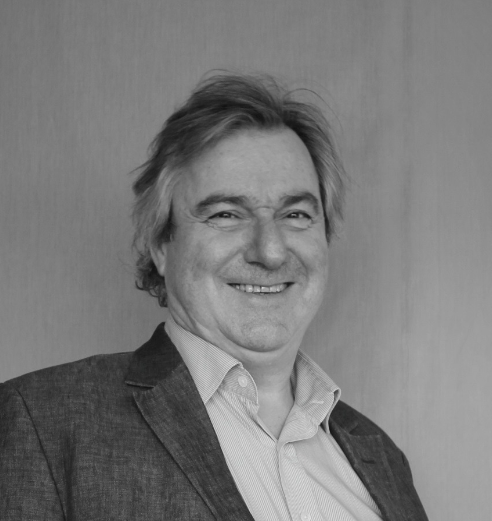
\includegraphics[scale=0.5]{images/pierre}

“Avec l’idée fondatrice d’apporter une offre globale de services respectueuse de l’homme et de l’environnement sur le marché de l’industrie chimique, EcoMundo est devenu, en 10 ans, un acteur incontournable du secteur. 

Fruit d’une longue expérience professionnelle dans l’industrie chimique, d’un profond attachement aux valeurs de travail en entreprise, d’amitié et de performance, nous avons intégré au fil des années l’ensemble des savoir-faire autour de la réglementation sur les substances chimiques pour devenir un partenaire unique et compétitif de la chaîne industrielle.

Notre croissance continue nous engage de façon constante vers de nouveaux défis avec, entre autres, le développement de nos différentes filiales au Canada, en Corée du Sud et en Espagne. La recherche de synergies permanentes entre nos différents pôles sont plus que jamais un gage de flexibilité et d’efficacité en adéquation avec nos flux de commandes. Nos équipes s’affairent à co-construire au quotidien des projets au service d’un bien vivre collectif.

Acteur au cœur du tissu économique et écologique, nous mettons tout en œuvre pour accompagner la réalisation de projets industriels exigeants tout en gardant l’esprit originel d’une entreprise à dimension humaine, innovante et accessible, dans les pas d’une ambition intacte, celle de construire autrement.”


Pierre Garçon
Founder

\subsection{History}
\begin{itemize}
\item \textbf{2001}

Pierre Garçon participates in the European projects EDIT and ECODIS on the traceability of hazardous substances and environmental data.

\item \textbf{2007}

Entry into force of the REACH Regulation: Europe establishes means to ensure a high level of protection against risks related to substances. Pierre Garçon and Jean-Raphaël Miron join forces to found the company EcoMundo. The initial core activity: compliance with REACH.

\item \textbf{2010}

After 2 years of development, launch of SaaS software solutions dedicated to industrialists for mastering compliance with REACH.

\item \textbf{2011}

EcoMundo's team grows from 2 to 27 employees.

\item \textbf{2012}

Opening of a new office in Vancouver, Canada, to provide regulatory expertise to international companies.

\item \textbf{2013}

EcoMundo diversifies its areas of regulatory expertise and meets the industry's new needs related to the European regulations on Cosmetics and Biocides.

\item \textbf{2014}

EcoMundo increases its capacities and becomes one of the main European actors concerning REACH authorization dossiers.

\item \textbf{2016}

Launch of the COSMETIC Factory software solution that revolutionizes cosmetic regulatory management. It notably allows for the automation of DIP creation.

\item \textbf{2017}

Following a fundraising round, EcoMundo's capital is raised to 1 million euros. The number of employees continues to increase!

\item \textbf{2018}

Opening of a new branch in Seoul, South Korea, mainly dedicated to cosmetics. The Vancouver office is transferred to Montreal, Canada.

\item \textbf{2019}

Opening of a new branch in Barcelona, Spain.

\item \textbf{2020}

Opening of a branch in London, United Kingdom. The teams now consist of 43 employees in Paris, 3 in Montreal, 4 in Seoul, and 2 in Barcelona. Finally, the offices in Paris are renovated to provide employees with an environment in line with our values.
\end{itemize}
\section{Organizational framework}
This section provides a consice overview of Ecomundo's internal organization, delineating the functional departments and collaborative networks that constitute the company's framework.
\subsection{Human Resources}

The Human Resources department plays a pivotal role in managing and developing the organization's workforce. It is responsible for various activities, including recruitment, talent acquisition, training and development, employee relations, performance evaluation, and compensation management. By ensuring a skilled and motivated workforce, the Human Resources department contributes to the overall success and growth of Ecomundo. The director of this department is the Chief Financial Officer Simon PICCA.

\subsection{Corporate Communication}

Effective communication is crucial for any organization's success, and Ecomundo recognizes this importance by maintaining a dedicated Corporate Communication department. This department is responsible for managing both internal and external communication activities. It encompasses public relations, media relations, branding, and corporate messaging. Through strategic communication initiatives, the Corporate Communication department promotes Ecomundo's brand image, enhances stakeholder relationships, and facilitates the dissemination of information to employees and external audiences. The director of this department is the Marketing and Communication Director Laure SCHMITT.

\subsection{Scientific Expertise}

As a company specializing in environmental sciences, Ecomundo places great emphasis on scientific expertise. The Scientific Expertise department consists of subject matter experts who possess in-depth knowledge and experience in various scientific domains. These experts provide valuable insights, technical guidance, and scientific support across different projects and initiatives undertaken by Ecomundo. Their contributions ensure that the organization's activities align with the latest scientific advancements and industry best practices. The director of this department is the Chief Scientist Officer Benoît SOTTON.

\subsection{Regulatory Affairs}

Compliance with regulations and standards is of paramount importance for Ecomundo. The Regulatory Affairs department is responsible for monitoring and ensuring adherence to applicable regulations and standards. This includes staying updated on regulatory changes, preparing and submitting regulatory documentation, conducting regulatory assessments, and liaising with regulatory bodies. By actively managing regulatory affairs, Ecomundo demonstrates its commitment to maintaining compliance and upholding the highest ethical and legal standards. The director of this department is the Legal Affairs Director and Head of Authorisation Béatrice ZAREMBA.

\subsection{Sales}

The Sales department serves as the key driver of revenue generation for Ecomundo. It is responsible for identifying and acquiring new customers, nurturing existing client relationships, and promoting the organization's products and services. The Sales team collaborates closely with other departments to understand customer needs, develop tailored solutions, and provide exceptional customer experiences. By effectively positioning Ecomundo's offerings in the market, the Sales department contributes to the organization's growth and market competitiveness. The director of this department is the Chief Operation Officer (COO) Fangcun ZHOU.

\subsection{Innovation \& Software}

To stay at the forefront of technological advancements, Ecomundo maintains an Innovation \& Software department. This department fosters a culture of innovation within the organization by exploring emerging technologies, conducting research, and developing software solutions. The Innovation \& Software team collaborates with other departments to identify opportunities for process improvement, streamline operations, and enhance productivity. Through its innovative approach, this department enables Ecomundo to adapt to changing market dynamics and deliver cutting-edge solutions to its clients. The director of this department is the Chief Operation Officer (COO) Fangcun ZHOU.

\subsection{IT}

The IT department plays a critical role in managing Ecomundo's information technology infrastructure. It ensures the smooth operation of computer systems, networks, and software applications throughout the organization. The IT department is responsible for system administration, network management, cybersecurity, technical support, and data management. By maintaining a robust and secure IT infrastructure, this department enables efficient and secure access to information, facilitates effective communication, and supports the organization's overall business operations. The director of this department is the Co-Founder and the Chief Technical Director Jean-Raphaël MIRON .


\subsubsection{DevOps}

The DevOps sub-department combines software development and operations to enable efficient and reliable software deployment, infrastructure management, and continuous integration and delivery. DevOps professionals collaborate with software developers, system administrators, and quality assurance teams to streamline development cycles, automate processes, and improve overall software reliability and performance.

\subsubsection{R\&D (Research \& Development)}

The R\&D sub-department within the IT department focuses on exploring new technologies, conducting research, and developing innovative solutions. R\&D professionals work closely with other departments to identify opportunities for technological advancements, prototype new features, and enhance existing software solutions. Their research-driven approach ensures that Ecomundo remains at the forefront of technological innovation within the environmental sciences domain.
During my stay in Ecomundo, I was part of this department, under the supervision of Jean-Raphaël MIRON the Chief Technical Director and Anna PERFETTO the AI Engineer.

\subsubsection{Quality}

The Quality sub-department is responsible for ensuring that software and systems developed within Ecomundo meet established quality standards. Quality professionals conduct comprehensive testing, implement quality assurance processes, and adhere to best practices throughout the software development lifecycle. Their efforts contribute to the delivery of reliable, user-friendly, and high-quality software solutions to Ecomundo's clients.

\subsubsection{Data}

The Data sub-department handles data management within the IT department. Data professionals are responsible for data analysis, database administration, data integration, and data security. They collaborate with other teams to ensure data integrity, facilitate data-driven decision-making processes, and maintain the confidentiality and privacy of sensitive information. Through effective data management, this sub-department provides valuable insights and supports evidence-based decision making within Ecomundo.

\subsubsection{Dev}

The Dev sub-department focuses on software development within the IT department. Dev professionals are responsible for writing and maintaining code, implementing new features or enhancements, and ensuring software solutions align with project requirements and specifications. They collaborate with other teams to develop robust and scalable software applications that meet the needs of Ecomundo's clients.

\subsubsection{LAB}

The LAB sub-department is involved in testing and quality control activities within the IT department. LAB professionals conduct experiments, analyze results, and ensure compliance with regulatory standards and best practices. Their expertise in quality control and testing procedures ensures that software solutions developed within Ecomundo are reliable, accurate, and in compliance with industry standards.

\subsubsection{Product}

The Product sub-department works closely with other teams within the IT department to oversee the development and management of software products. Product professionals collaborate with stakeholders to define product requirements, prioritize feature development, and ensure alignment with customer needs and market trends. Their role encompasses product strategy, roadmap planning, and product lifecycle management.

\subsection{My position}
During my internship at Ecomundo, I was assigned as an AI Engineer Intern inside the  IT-R\&D department, under the supervision of both Chief Technical director Jean-Raphaël MIRON and AI Engineer Anna PERFETTO.
\section{Internship objectives}
The main objectives of this internship are to design, develop, test and document innovative solutions that adress business and R\&D challenges. The area of focus includes designing and improving rule-based expert systems that leverage knowledge and logic to provide answers to complex tasks that are traditionally done by a human. Additionally, developping AI solutions in different areas using Natural language processing and Machine/Deep Learning. Once these AI solutions are designed and developped, the next crucial step is to deploy them effectively. This envolves ensuring their quality and integrating them into the existing technical infrastructure of the organization. Rigourous testing procedures, such as unit testing, integration testing and performance testing are employed to validate the reliability and efficiency of the solutions. And to keep the projects well defined for future references, we worked on writing well documenting our work in order to provide clear intructions and guidelines for the code, deployment steps, maintenance and error handling.

\section{Software}
\subsection{Cosmetic Factory}
\subsection{SDS Factory}
\chapter{Methods and tools}
\thispagestyle{empty}
\section{Transformers}
Transformers\cite{NIPS2017_3f5ee243} have been introduced in 2017 to replace the Recurrent Neural Networks architectures using self-attention mechanisms and the encoder-decoder architecture that hugely improved the performance of such models.

\subsection{Word Embedding}
Word embedding is the approach that allows computers to understand words by converting them into numeric vectors. In this space of vectors, words with similar meanings have close or similar representation. One famous algorithm frequently used is Word2Vec\cite{mikolov2013efficient}. The basic idea is that two words are considered similar if they are often used in similar context.

\subsection{Attention}
The attention mechanism allows the model to effectively capture relevancy between words in a sentence by calculation attention scores. The scores are calculated using the dot product between each word and the target word of interest. Softmax function is then used to transform the scores into `meaningful` weights that help the model emphasis important words while de-emphasising less significant ones. This mechanism gives the model the superpower of understanding the contextual nuances and relationships between words, which is the ideal goal for Natual Language processing tasks.


\subsection{Encoder-Decoder Architecture}
\subsubsection{Encoder}
In the encoder, the input words are first embedded into a high-dimentional vector space. then we add to these embeddings to capture the position of the token in the sequence. Each token is transformed into three vectors: Query (Q), Key (K) and Value (V). This transformation is performed using learnable weight matrices:
$$Q = X \cdot W_{Q}$$
$$K = X \cdot W_{K}$$
$$V = X \cdot W_{V}$$
Self attention scores are then calculated as the dot product. For query vector $q_{i}$ and a key vector $k_{j}$, the attention is: 
$$Attention(q_{i},k_{j}) = q_{i} . k_{j} / \sqrt{d}$$ 
With d the dimention of the key vectors.

Attention weights are simply the softmax of the attention weights: $$\alpha_{ij} = softmax(Attention(q_{i},k_{j})$$

The final output of the attention mechanism is obtained by taking the weighted sum of the value vectors V.
$$AttentionOutput(q_{i}) = \sum_{j}\alpha_{ij} V_{j} $$
\subsubsection{Decoder}
At the decoder level on the other hand, attention is used in two ways, a self-attention and an encoder-decider attention. The first one works by doing the exact same thing as the encoder, however it employs masking that prevents the decoder from accessing future positions. The Second allows the decoder to attend relevant parts of the input while generating the output. The encoder's output serve as as the key value vectors, and the query vectors are derived from the state of the decoder.

\subsection{HuggingFace}
Huggingface\cite{huggingface} is an opensource known for their contributions for the transformers library, one of the most used libraries for NLP and AI tasks in general. 
Transfomers library provides a wide range of pre-trained models for multiple purposes such as text classification, NER, text generation, translation, etc... It is build on top of the PyTorch and TensorFlow frameworks.
Huggingface has played an important role in democratising NLP and making it more accessible, they provide really powerful language models such as BERT, GPT and RoBERTa that can either be used directly, or for transfer learning. They also provide a large range of datasets that can be used for model fine-tuning for various specific tasks.

\subsection{OpenAI \& GPT}
\subsubsection{Generative Pretrained Transformers}
GPT models are Language models that have been trained on huge amounts of data such as books, web data and human conversations for the purpose of developping a general understanding of the language. 
\paragraph{GPT-1}
It all started with GPT the first release by OpenAI\cite{openai} in 2018. It had 117 million parameters. It was mainly trained to be able to correctly predict the next word in a sentence. It suffered from the lack of understanding when given a longer context which resulted in incoherent outputs.
\paragraph{GPT-2}
In 2019, OpenAI released GPT-2 with 1.5 billion parameter, about 10 times larger than its predecessor. It outperformed the first gen model in the ability of generating coherent text. Due to concerns for misuse, the use of this model was initially very limited. Which will lead OpenAI to perform different types of trainings for their future models.
\paragraph{GPT-3}
In their paper ``Language Models are Few Shot learners''\cite{brown2020language}, it was demonstrated how a large model like GPT 3 with a 175 billion can easily learn and adapt to new tasks only using few examples (few-shot learning). Obviously, it also demonstrated better language understanding and impresive performance on multiple NLP tasks such as summarization, question answering and translation
\section{LangChain}
With large language models emerging as a revolutionary technology, Langchain\cite{langchain}, an opensource framework, allows developpers to build applications that were near impossible to make before. Some good examples of those applications are Document Question Answering, Chatbots, Agents.
\section{Ensemble Learning}
Ensemble learning is a Machine Learning technique that combines multiple base models in order to produce a more powerful model that can achieve higher accuracies. By combining the predictions of each base model, we can capture the diverse knowledge and expertise of these models which leads to an improved overall performance. In order to achieve the most optimal results, many aspects need to be considered:
\subsection{Diversity of Base models}
When we talk about ensemble learning, we usually gather multiple models that are considered weak learners. These models have, individually, slightly better performance than random prediction. In order to squeeze the maximum out of this method, the models should be diverse. Diversity ensures that each model brings unique information and makes different errors, reducing the chances of the resulting model being biased or the results being fluctuated by a single model's shortcomings. We can push this further by feeding each model a different subset of our dataset.
\subsection{Aggregation}
Each model in Ensemble learning should predict his own output, then the final result is the aggregation of the multiple outputs. It can be a voting-based method which involves casting votes from each model. The voting can be either HARD, which basically means the majoritarian result is the final result. Or it can be SOFT, which is a weighted vote based on Confidence intervals.
The other way to do it is by averaging the outputs. In this method we take the weighted average of the predictions from all the underlying models to get the final prediction.
\section{Gradient Boosting}
Gradient boosting is a type of ensemble learning. The key idea behind it is to iteratively build an ensemble of weak prediction models, where each sub model corrects the errors made by the other models. This iterative process follows the gradient of the loss functions.
A very known model for Gradient Boosting is XGBoost:
\subsection{XGBoost}
A Known Gradient boosting machine learning model for his performance and versatility in solving multiple supervised learning tasks. It works as follows:
\begin{enumerate}	
\item XGBoost starts by initializing a set of weak base models, usually decision trees called a regression tree. Each tree is trying to correct the mistake made by the previous tree. These trees are build sequentially.
\item To define whether the model is performing well, and to guide it in the right direction, a metric or Objective function needs to be defined and optimized during the training process. It is composed of a loss function and a regularization term.
\item The model then computes the gradients of the loss function. It also computes the Hessian matrix to get further infromation about the curvature of the loss function.
\item The gradients and hessian values are used to determine the best splits when constructing the trees. Each branch is added based on the evalution of these splits.
\item Regularization penalties are added in order to prevent overfitting and control the complexity of the model to keep it simple. Prunning is also added at the end to further improve the performance and generalization of the model.
\item XGBoost uses early stopping by monitoring the performance of the model on the validation set and stops the learning process when the performance starts to degrade.
\end{enumerate}
\chapter{Projects}
\thispagestyle{empty}
\section{Challenge Test Predictions}
\subsection{Presentation of the project}
All creams, foundations, and shampoos that become tomorrow's BEST SELLER are the result of a long Research \& Development (R\&D) process. Before being launched into the market, they undergo microbiology tests, which can make or break their success. If they pass the microbiology tests, it will be a great achievement. If they fail, it will be a nightmare for the formulators who must adjust their formulations to turn their aspirations into reality.

Help has arrived from Cosmetic Factory, a PLM cosmetic software that assists R\&D laboratories in speeding up the launch of new cosmetic products. In partnership with the Occitane Group, Ecomundo has developed an Artificial Intelligence (AI)-powered solution to anticipate the outcomes of the Challenge Test (CT). It serves as an intelligent formulation aid for cosmeticians, and was unveiled during the Cosmetic 360 Conference in October 2022. 
What is a Challenge Test? The Challenge Test is a mandatory pre-market test required by regulations, based on the ISO 11930 method. It involves inoculating a particular concentration of bacteria, such as Escherichia coli, Candida albicans, Staphylococcus aureus, etc. To pass the test, a specific log reduction in the number of microorganisms recovered must be achieved at designated intervals, typically after 2, 7, 14, and 28 days.
\begin{figure}[H]
		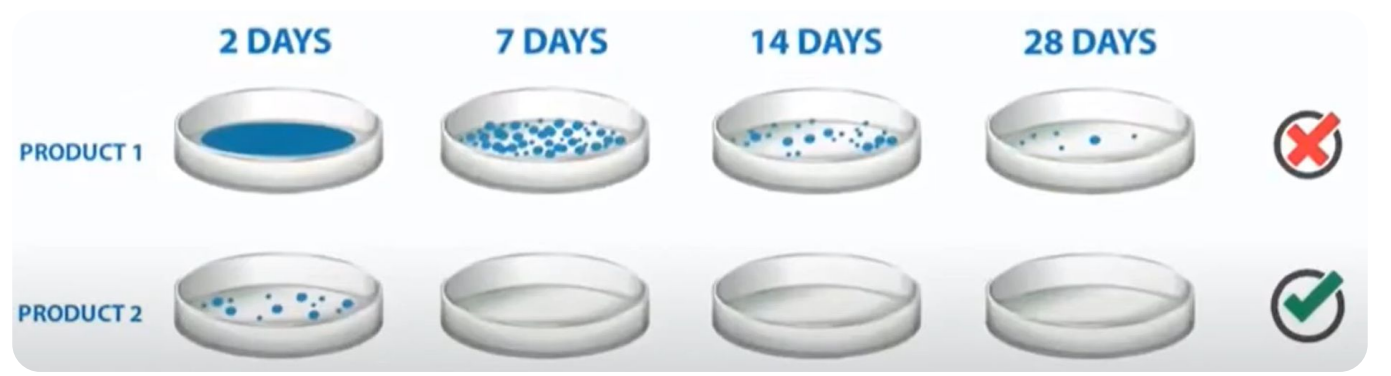
\includegraphics[width=\textwidth]{images/CT}
	\caption[Challenge Test]{CT}
\end{figure}

If the specified criteria are not met, as was the case with PRODUCT 1, cosmeticians are required to reformulate and test again until they develop a product that passes the CT, like PRODUCT 2. As a result, one can imagine the laborious nature of the process, as well as the waste of time and resources involved. This is where artificial intelligence comes to the rescue, with its predictive capabilities.

\subsection{How it is currently done}
EcoMundo has developed a hybrid AI solution, which combines an expert system (ES) and machine learning (ML) that predicts the result of the CT, in other words the efficiency of the conservation system. 
At the moment the solution has been implemented in Cosmetic Factory in the Formulas module, in the Prediction wizard (kyoto server).
\begin{figure}[H]
		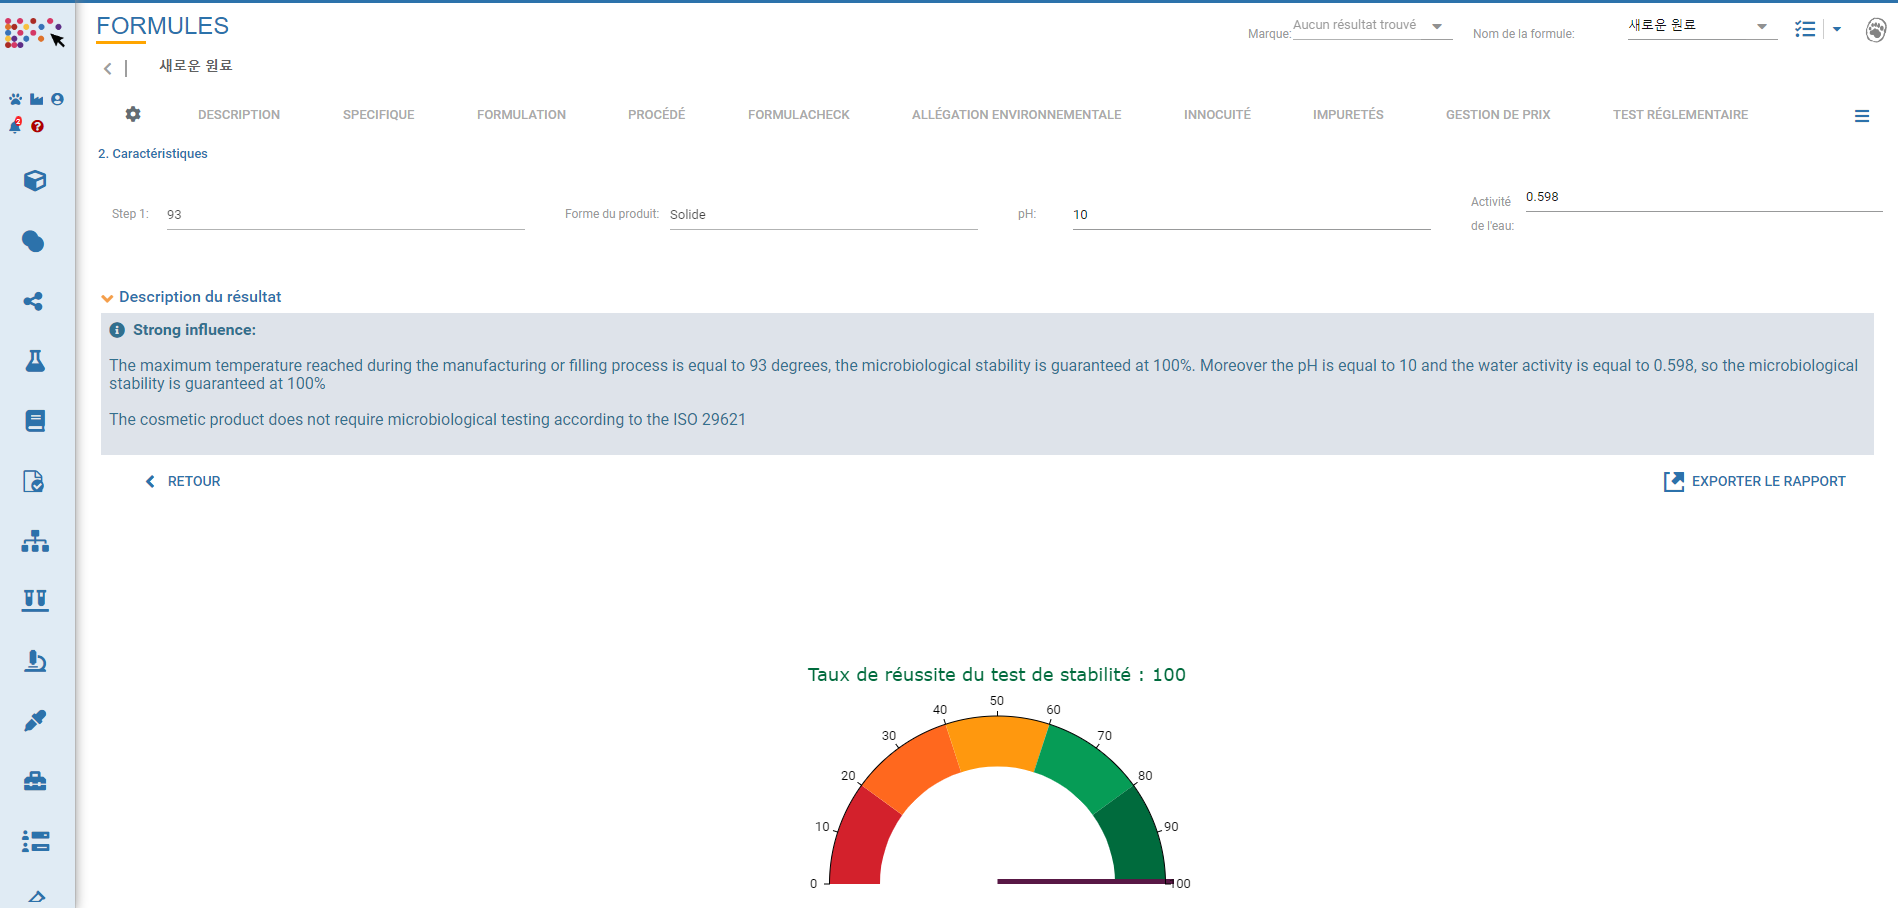
\includegraphics[width=\textwidth]{images/kyoto}
	\caption[Cosmetic Factory Interface for CT]{CF interface}
\end{figure}

To develop the hybrid AI solution we started to study the criteria influencing the risk of microbial contamination. The pH, which measures the acid or basic character of a solution, the water activity that quantifies the free water available to assure growth of microorganisms. Moreover, some raw materials are known to create a hostile environment for the survival of microorganisms like alcohols, inorganic solvents, humectants, inorganic salts, acid and bases. The formulation processes may have an influence on the microbial protection like temperature, incorporation order of ingredients, time of homogenization. And eventually the physical state, if our cosmetic product is a solid, powder, foam etc..
A hybrid system benefits from the reasoning and explanation of the ES, as well as the learning and generalization potential of ML algorithms, which determines an effective and efficient model. 
This allows users (cosmeticians, formulators, etc..) to understand the prediction, along with the scientific and regulatory reasons behind it. Indeed, the system provides suggestions for improvement, making this solution a useful and reliable formulation support and optimization tool to achieve the success of the challenge test immediately. 
How is the pipeline structured? The data are feeded to the ES which starts to assign success rate of the CT according to the rules codified in regulation, namely the ISO29621 and based on experimental results published in literature. These rules concern the empiric criteria influencing the risk of contamination based on certain values of pH, water activity, temperature etc. 
Thereafter, the ES calls the ML to have its success rate. We trained different ML algorithms, but the one that gave the best results is the decision tree applied on the set of ingredients present in the formulas. The result coming from the ML is eventually weighted by the expert system together with the other results, to give finally to the user the success rate of the challenge test.

\begin{figure}
		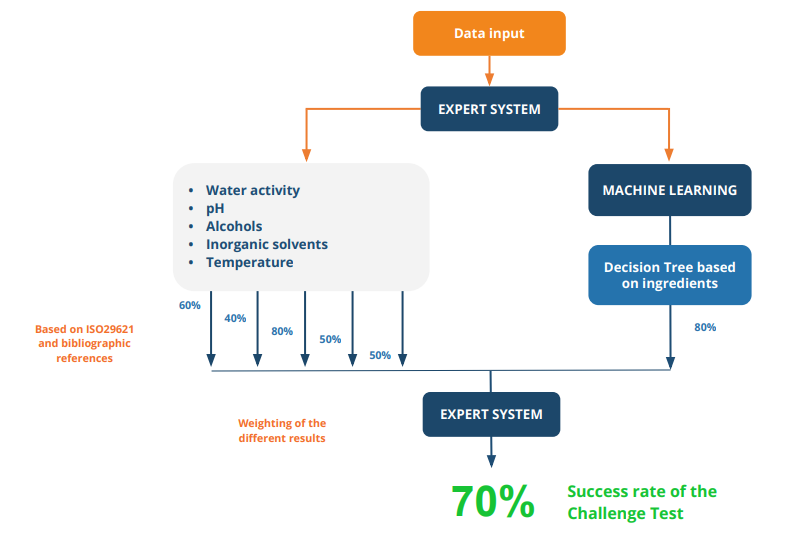
\includegraphics[width=\textwidth]{images/ctFlow}
	\caption[WorkFlow of CT prediction in CF]{CT flow}
\end{figure}


\begin{figure}
		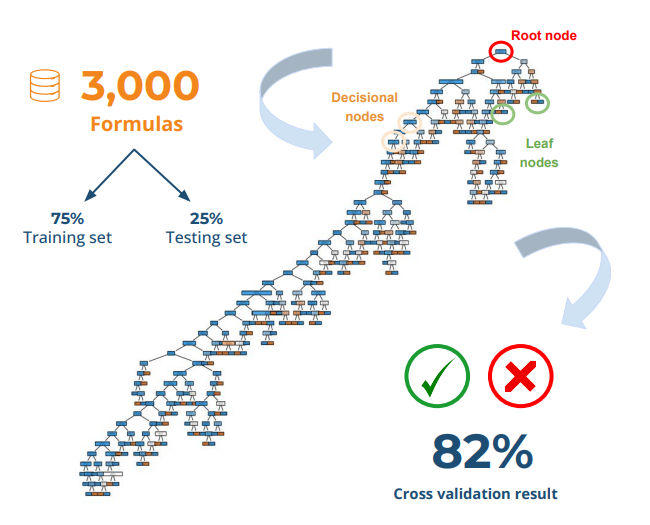
\includegraphics[width=\textwidth]{images/binaryTree}
	\caption[Current Decision Tree for CT prediction]{Decision tree}
\label{Decision tree}
\end{figure}
The ML algorithm chosen is the supervised binary classification, see the decision tree \ref{Decision tree} , trained on the ensemble of ingredients and their concentration. 3000 formulas furnished by the Group Occitane have been selected and have been divided into 2 sets: a training set which represents 75\% and the rest has been used as a testing set.
The decision tree at the end gives as answer Yes/No, in other words it is able to say if each formula passes or fails the CT, with a precision of around 80\%.

The learning database is composed of formulas, descriptors like pH, water activity and temperature, etc.., which somehow affect the CT results, and of course the CT results. Here, you can find the data conceptual model (DCM) to have a complete vision of the information necessary to train the models.
\subsection{New solution}
The new solution is based on ensemble learning. By utilizing multiple models instead of just the decision tree, we will be using XGBoost, Random Forest and a Neural Network. Before the pseudo code presentation, I am presenting in the next subsection the datasets that have been used, the problems with it and how we managed to overcome them.
\subsubsection{Datasets}
These datasets have been provided by L'Occitane \ref{MCD Challenge Test}:
\begin{itemize}
\item \textbf{ECO\_liste des formules avec désignation:} contains list of codes of chemical formulas as well as the type, for example a cream, oil, scrub etc..
\item \textbf{ECO\_formule avec element tech:} Contains the formula code and its corresponding challenge test result.
\item \textbf{ECO\_formule avec liste INCI:} Contains the formula code, ingredients and their corresponding concentration.
\item \textbf{ECO\_formule avec code protocole:} Contains for each formula code, its corresponding protocol code. 
\item \textbf{ECO\_code protocole avec liste des codes étapes:} Each protocol of the last table, has many steps. Each step has its own code.
\item \textbf{ECO\_liste des codes étapes avec les conditions:} On each step, some conditions must be respected. Those conditions are in this table like temperature, time with each condition referred to as a code.
\item \textbf{ECO\_formule avec liste MP:} Table that contains for each formula the raw materials in it and their concentrations.
\end{itemize}
\paragraph{Remarks and problems about the datasets}
\begin{itemize} 
\item CODEMAT and CODEART are the same thing.
\item INCI represents one ingredient.
\item Raw Material is composed of multiple INCIs (ingredients)
\item Total number of Formulas is 7369, though only 5303 have CT results. Out of the 5303, only around 4000 formulas we have their exact compositions with the concentrations. 
\item Usually, the tests are positives because many hours are spent on making sure the product passes it. This leaves us with a very unbalanced dataset of around 90\% of the data have the label "YES", while only 10\% did not pass.
\item Not all raw materials have the same INCIs, so we have to put all the INCIs in columns and have it at 0 concentration if doesn't exist in the formula. This has left us with a large dataset column wise and it's very sparse ( around 80 percent of the values are zeros).
\end{itemize}
\begin{figure}[H]
		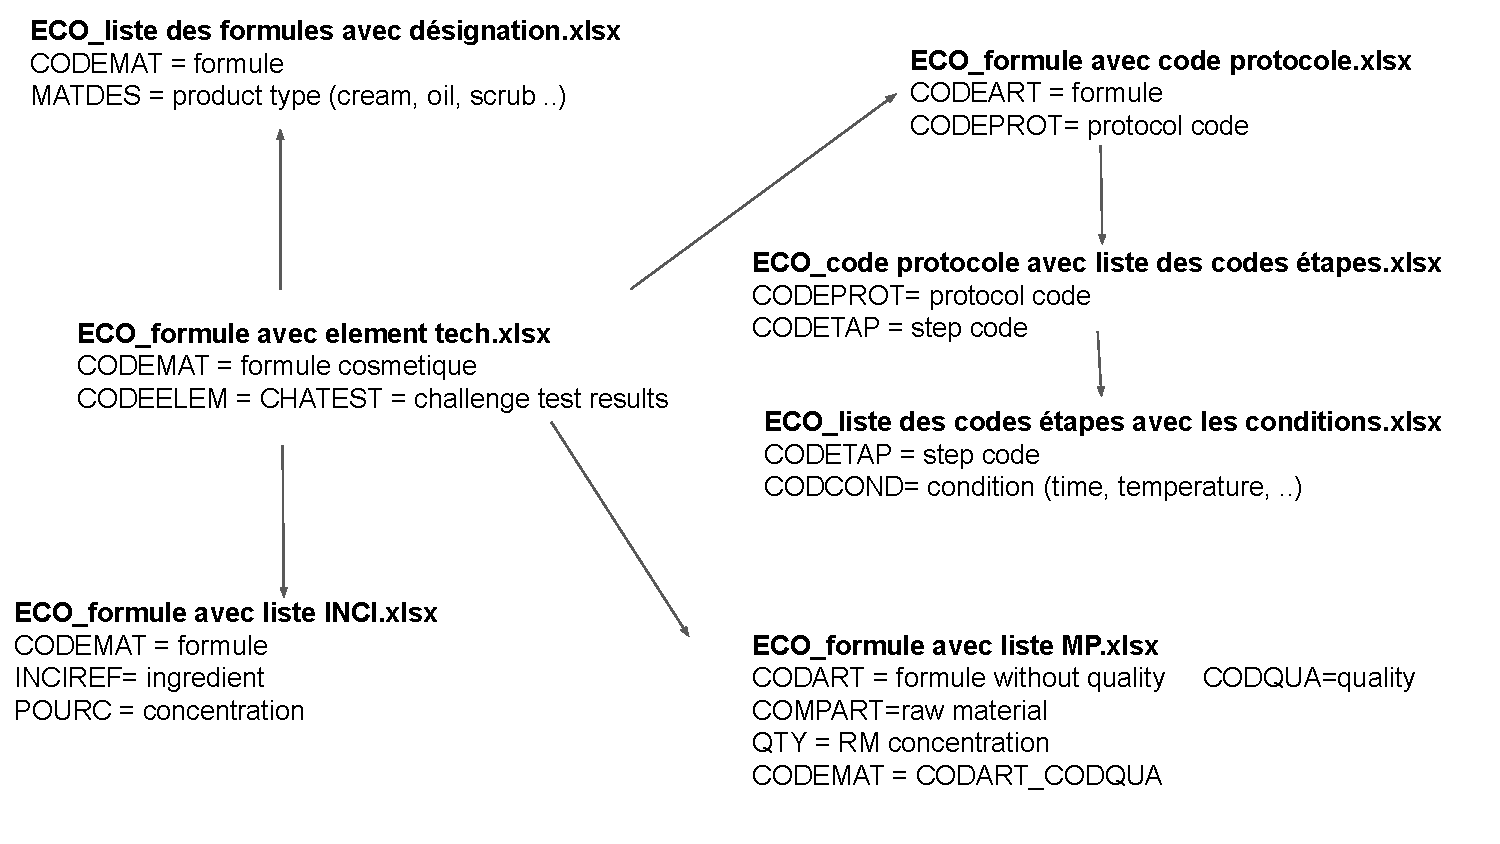
\includegraphics[width=\textwidth]{images/MCD_CT}
	\caption[MCD for L'Occiatane]{Datasets L'Occitane}
\label{MCD Challenge Test}
\end{figure}
To tackle these problems, first we needed to do a startified split on the dataset in order to well train it. Then imperatively use PCA in order to reduce the size of the dataset.
(code is not included in the report, will be presented live).

\subsection{ML Pipeline and Deployment Architecture}

Following the figure \ref{ML Pipeline}, this is how the ML pipeline is structured:
\begin{enumerate}
\item We have implemented a robust data collection mechanism to gather the required data from the EcoMundo database using SQL scripts. The collected data is then transformed into a CSV file for further processing.
\item For now, we have used a Google Colab notebook, where we perform extensive preprocessing on the collected data to ensure it is in a suitable format for ML model training. Using the pandas library, we create a structured dataframe. We then employ scikit-learn and TensorFlow libraries to train various ML models. Through optimization and fine-tuning techniques, we enhance the model's performance.
\item To integrate the ML model into the existing Cosmetic Factory software, we have designed and developed an AI application using the Django framework. This application is called when there is no response from the Rule Engine. Through a REST API, a Java controller in the backend is called, allowing communication between the ML model and the software.
\item We have implemented a mechanism for real-time inference, enabling the ML model to make predictions in real-time. The ML model's predictions are integrated with the existing software's logic. This process involves making API calls to retrieve answers, which are then sent to the Java controller and displayed in the application's front-end.
\item We have set up a manual periodic fine-tuning process to retrain the ML model using new data from the EcoMundo database. By incorporating user feedback and leveraging the latest data, we continuously improve the model's accuracy and effectiveness.

\end{enumerate}
\begin{figure}[H]
		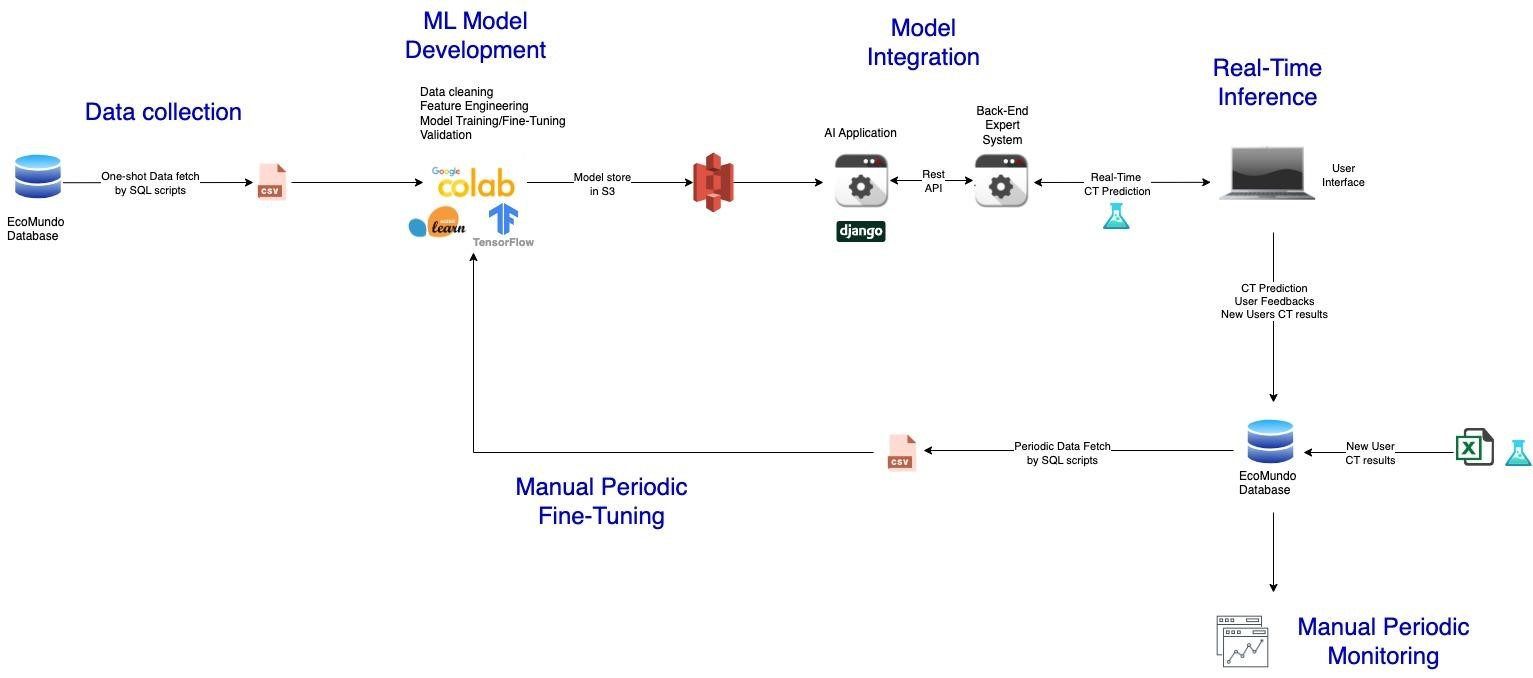
\includegraphics[width=\textwidth]{images/ctDeploy}
	\caption[ML Pipeline]{ML Pipeline}
\label{ML Pipeline}
\end{figure}
\subsection{Results and Comments}
\subsubsection{Metrics}
Because we are working on a binary classification, precision alone is not a good metric for how performant the model is. This metric only computes how many times a model made a correct prediction across the entire dataset. Recall on the other hand measures how many of the positive class samples present in the dataset were correctly identified by the model.
F1-score is the best for this use case, since it's compatible with unbalanced datasets and it combines both recall and precision. 
$$ F_1 = 2 * \frac{precision * recall }{precision + recall} $$

Another Metric that we have used is the ROC AUC score. It reflects on how efficient the model is. The higher the Area Under the Curve, the better model's performance at distinguinshing between the two classes.

\subsubsection{Results}
\begin{figure}[H]
		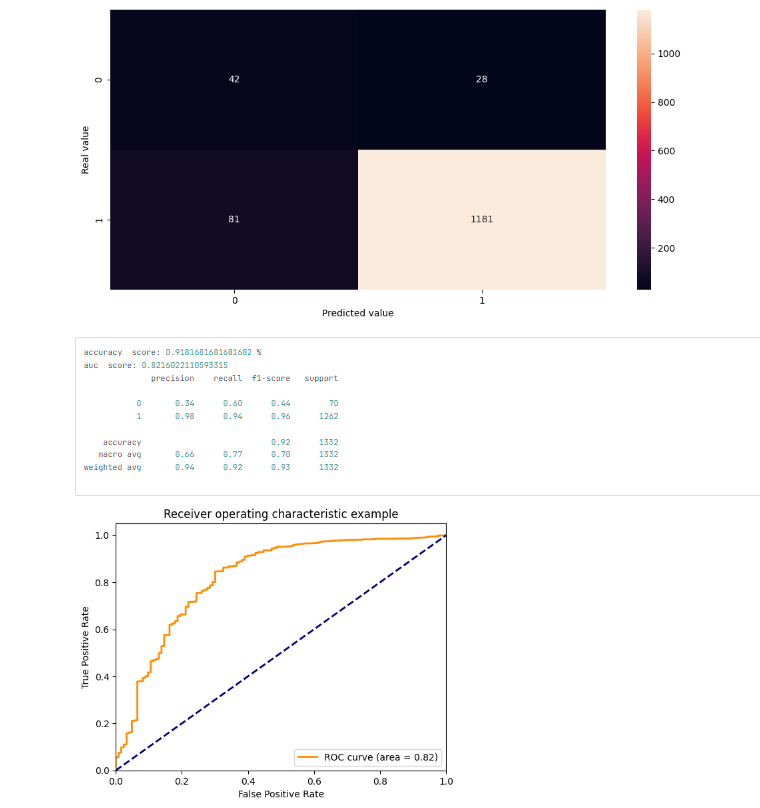
\includegraphics[width=\textwidth]{images/xgboost}
	\caption[XGBoost Confusion Matrix, AUC]{XGBoost Confusion Matrix, AUC}
\label{xgboost}
\end{figure}
\begin{figure}[H]
		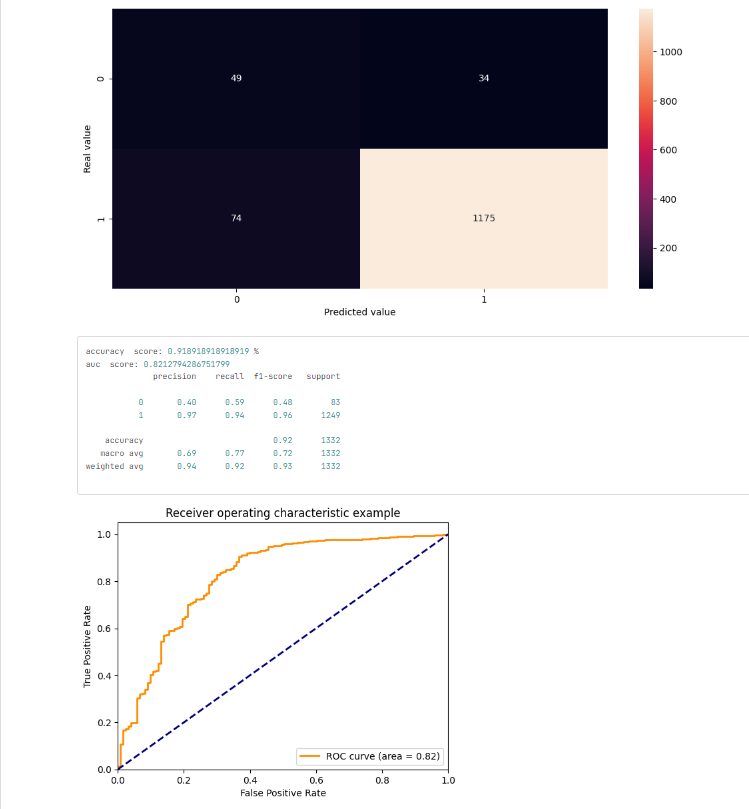
\includegraphics[width=\textwidth]{images/randomforest}
	\caption[Random Forest Confusion Matrix, AUC]{Random Forest Confusion Matrix, AUC}
\label{randomfor}
\end{figure}
\subsubsection{Comments}
The result that we got on the inference of these two models have been enough

\begin{figure}[H]
		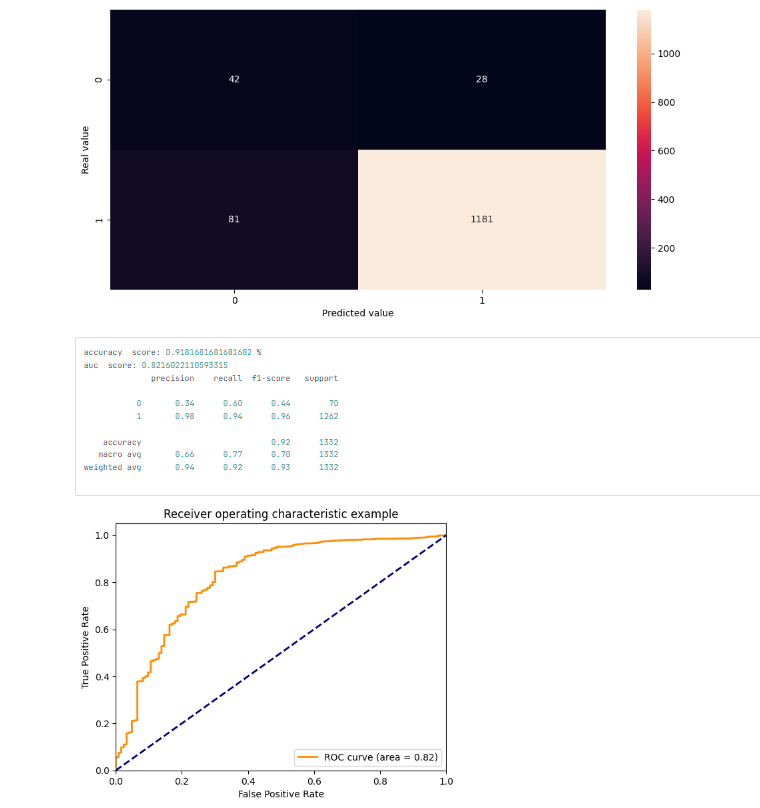
\includegraphics[width=\textwidth]{images/xgboost}
	\caption[XGBoost Confusion Matrix, AUC]{XGBoost Confusion Matrix, AUC}
\label{xgboost}
\end{figure}
\section{SDS Reader}

\subsection{Presentation of the project}
Currently called PDF Reader, is an application made by Ecomundo specifically for Safety Data Sheets:
\subsubsection{What is an SDS?}
Safety Data Sheet, also known as Material Safety Data Sheet (MSDS), is a very important document that provides informations about the hazards and safe handling of a specific substance/mixture. Its main purpose is to ensure the safety of individuals who may use or come in contact with the substance in any settings. It it composed of sixteen sections:
\begin{itemize}
\item \textbf{Identification:} Identification of the substance/mixture on the SDS as well as the recommanded uses. It contains also the contact informations for the suppliers/manifacturers
\item  \textbf{Hazard Identification:} This section identifies the hazards of the substance/mixture presented in the SDS along with their appropriate warning informations
\item  \textbf{Composition/Information on Ingredients:} This section identifies the substance(s) contained in the product, their concentration and their hazard classification.
\item \textbf{First-Aid Measures:} Descriptions of the initial care that should be ginven by untrained responders to an individual who has been in contact with the chemical.
\item \textbf{Firefighting Measures:} Recommandations for fighting the fire caused by the chemical.
\item \textbf{Accidental Release Measures:} This section has recommandations on the appropriate responses to spills, leaks ro relases including containment and cleanup practices to minimize or ideally prevent exposure to the people and the environment.
\item \textbf{Handling and Storage:} Guidance on the best and safe practices of handling and storing the product.
\item \textbf{Exposure Controls/ Personal Protection:} In this section, the exposure limits, engineerings controls and personal protective measures are indicated.
\item \textbf{Physical and Chemical Properties:} This section identifies the physical and chemical properties of the substance/mixture
\item \textbf{Stability and Reactivity:} This section provides information about the reactivity hazards of the chemical and its stability information.
\item \textbf{Toxicological Informations:} Informations about the toxicological and health effects.
\item \textbf{Ecological Information:} This section provides information to evaluate the environmental impact of the substance(s).
\item \textbf{Disposal Considerations:} Guidance on proper disposal practices, recycling or reclamation of the substance(s) or its container and safe handling practices.
\item \textbf{Transport Information:} Guidance on classification information for shipping and transporting of hazardous substance(s) by road, air, rail, or sea.
\item \textbf{Regulatory Information:} Safety, health and environmental regulations specific for the substance/mixture that is not indicated anywhere else on the SDS.
\item \textbf{Other Information:} Indications about the preparation and revision date of the sds along with other useful information such as the changes that have been made compared to the last version. 
\end{itemize}
\subsection{How it is currently done}

\subsubsection{Get sections}
The old code is a static code that mainly starts by dividing the pdf into paragraphs. then go through each paragraph and detect where the sections are by comparing the words to the words that define sections in the SDSFactory database. For example you can have "SECTION" as the word splitting the document into sections, might also be "RUBRIQUE" if it's in French. It uses all possible words that are available in the database in the language of the SDS.
\subsubsection{Get Key-Value pairs}
Using Regular Expressions, the code then goes through each section and finds all the key value pairs that are mentionned in the PDF file. This is already problematic since there are inconsistencies of how a key value pair is shown in the file: It could be in the form of Key:Value, sometimes it's Key \\n Value.
\subsubsection{Match with Ecomundo Template}
Using the same static method of looking into the database, the code then goes through all the key value pairs and matches them with the Ecomundo Template of Keys. 
\subsection{Problems with the old way}
As it is very obvious, the static way of searching through the database for keywords, and expecting to have the exact same match is far from optimal. If we have an SDS with a different language then we have to recreate a table in the database for that exact same language, then fill it with all possible words for each key. For example the key "Product Name" can be in the pdf as "Product identifier" or just "Name", if we don't have these keys in the database, it will assume this data does not exist in the pdf.
We notice as well the workload of refreshing and updating the database frequently in order to keep it updated.
\subsection{New solution}
\subsubsection{Usage of Large Language Models}
The usage of large language models was first proposed as it will allow us to read the pdf and understand it then extract data from it. This method as demonstrated first by using ChatGPT and giving him texts in different languages from an SDS and providing him the keys to extract. Two major problems have arised from the proposition of using this method:
\paragraph{Security}
Sending PDF files of clients to OpenAI servers in North America for processing is not a straightforward procedure. The Technical directors were worried about data privacy of the clients even if SDS are not considered confidential in most cases. But as we will be using GPT models using the OpenAI api, and as a company, I suggested we contact sales and request to not store our sent data after the processing is done. It is a right that anyone can ask for when purchasing the api key\cite{openaiUP}.
\paragraph{Cost}
At the time of the first meeting 13th March 2023, the pricing for gpt-3.5-turbo model was 0.002 USD/1000 Tokens. The commercial team were not convinced of how cheap it is until I presented a proof of concept later on.
\subsubsection{Open-Source Large Language Models}
To tackle these two problems, I proposed to postpone the GPT api purchase while I dig deep into how we can use an opensource model. I started by looking into the models that are Open Source + Available for commercial use:
\paragraph{BERT and its derivatives}
The BERT model \cite{devlin2019bert} (Bidirectional Encoder Representations from Transformers) was introduced in 2018 by researchers at google. It achieved state-of-the-art performance on many NLP benchmarks. 

In my proposition to use open source models, BERT models came in as top results. BERT model was optimized when RoBERTa\cite{liu2019roberta} (Robustly optimized BERT) was introduced in 2019 which was optimized even more with the introduction of DeBERTa \cite{he2021deberta} (Decoding-enhanced BERT with disentangled Attention).

I started initially by using these models for question answering. The PDF file would be converted into a raw text fille, then fed to the model as context. Then I gave it the keys that I wanted to extract. DeBERTa Model was the best obviously, but still lacked in many areas:
\paragraph{Bad extraction}
The model was very inconsistent with the extractions, some keys would be perfectly extracted while other were not. The model also does not quite understand the structure of the page only from the raw text given to it as context.
Finetuning is always an option with these models, for the lack of time that I had with them on-site, and the deadline that we had for the end of June, we have proceded to the usage of other solutions.
\subsubsection{GPT}
OpenAI has made the model gpt-3.5-turbo available from their api for as cheap as 0.002 USD/1K tokens. To demonstrate the power of the model and how cheap it can be, I did a demo doing extraction of all key value pairs of an SDS page by page. It costs around 0.01 Euros per pdf of 13 pages. This has captured the attention of Christian FRENEUIL, the Software and Cloud services Sales Director, and pushed this project. 

\paragraph{First Version of the stable code: Non-Hybrid}
This code works as follows: 
\begin{enumerate}
\item Extract all key value pairs from each page. Keep a record of what sections are in that exact page, and save the latest one. For example if a page has Section 1 and Section 2, we save them both in an array, then we save the fact that section 2 was the latest. 
\item When we move to the next page, we check whether the page starts direclty with a section, then we assign the key values of that section to the corresponding key, if not we assume it's the Section 2 continued.
\item Group by Sections then send it to another controller in the application that will then match the key value paris from each section into the keys that we have.
\end{enumerate}
\begin{figure}[H]
		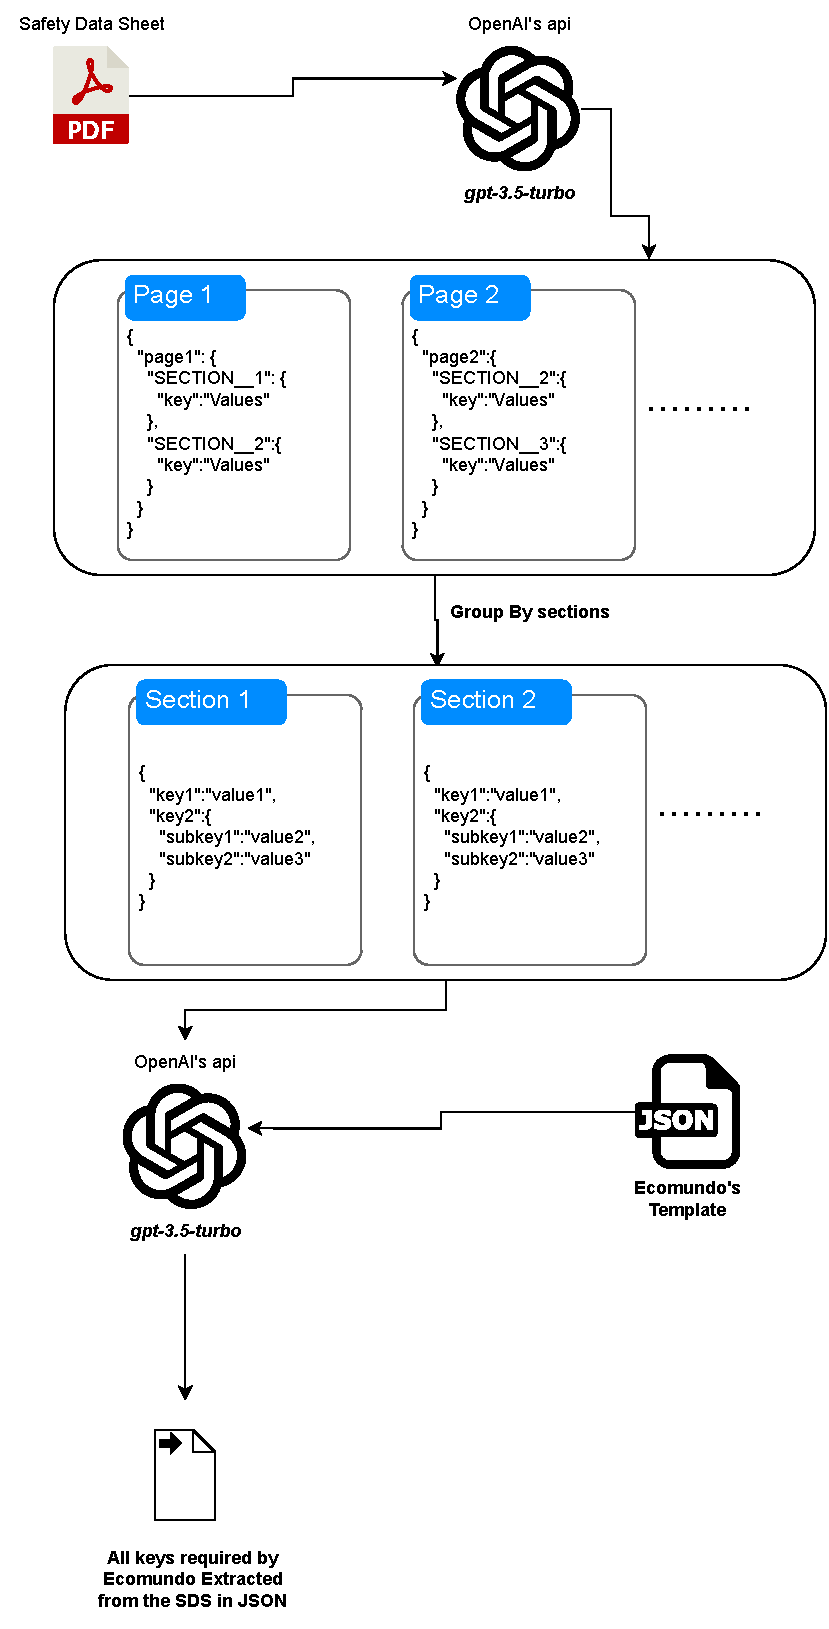
\includegraphics[width=\textwidth, height=\textheight/2, keepaspectratio ]{images/Non-Hybrid}
	\caption[How the Non-Hybrid code works]{Non-Hybrid}
\label{Non-Hybrid}
\end{figure}


\paragraph{Hybrid Version of the code}
As it is obvious in \ref{Non-Hybrid}, we are using OpenAI's api twice. The first extraction is taking an overhead task of detecting sections, that in some cases fail. To overcome this problem, we thought about using the existing PDFReader controller that splits the SDS into sections, and then use them directly for extraction and matching. This will give us Two benefits:
\begin{enumerate}
\item \textbf{Parallel extraction:} We will be able to parallelize the extraction for each section, and the extraction by Ecomundo's template for each section. Which means the complexity of this extraction will be the complexity of the longest Section. 
\item \textbf{Better Extraction:} Since we are focusing on only one task, the gpt model will work better with a one-goal instruction rather than multiple ones.
\end{enumerate}
\begin{figure}[H]
		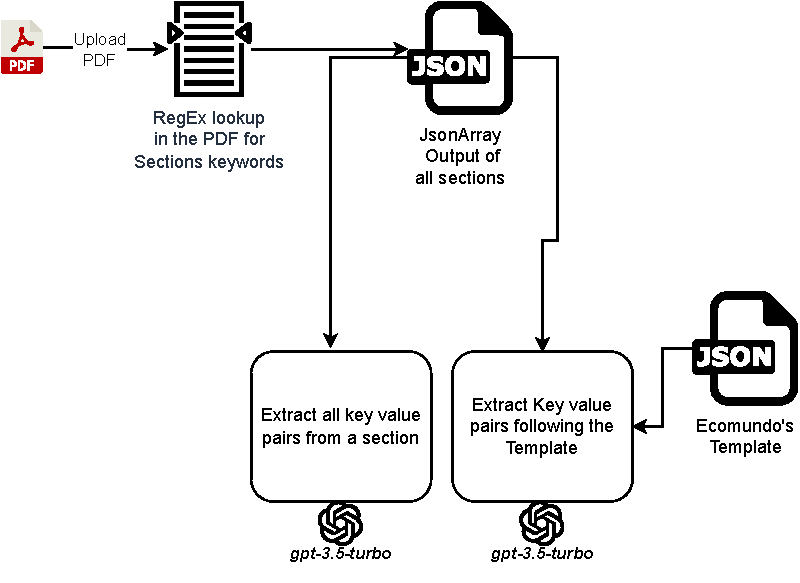
\includegraphics[width=\textwidth, keepaspectratio ]{images/hybrid}
	\caption[How the Hybrid code works]{Hybrid}
\label{Hybrid}
\end{figure}

\paragraph{Even More improvements}
To tackle problems relating to either: Size of the context (in our case the raw pdf text) and/or the quality of section extraction, I proposed a further architecture improvement. \ref{Hybrid++}
\begin{enumerate}
\item The pdf is loaded into the SDSReader interface, we first extract the text, if the text is empty, this means it's not a digital PDF. We then use PyTesseract OCR to extract the text.
\item Check for the quality of section extraction. If the length of the sections' list is not 16, we assume we did not correclty extract and we use the previous stable code. If it's till not 16 sections, we move to the langchain solution for the entire pdf proposed in \ref{chatbot}.
\item Assuming we had 16 sections, before the extraction, we need to check for the context limit of the prompt+the raw text. If we are in the context window of gpt-3.5-turbo, which is 4097 tokens, we are good. If not, we check if it's less than 16K tokens, then we use gpt-3.5-turbo-16k, which costs about 0.003 for input tokens and 0.004 for output tokens. If we are still outside this range, then we use LangChain solution but for only that exact section.
\end{enumerate}
\begin{figure}[H]
		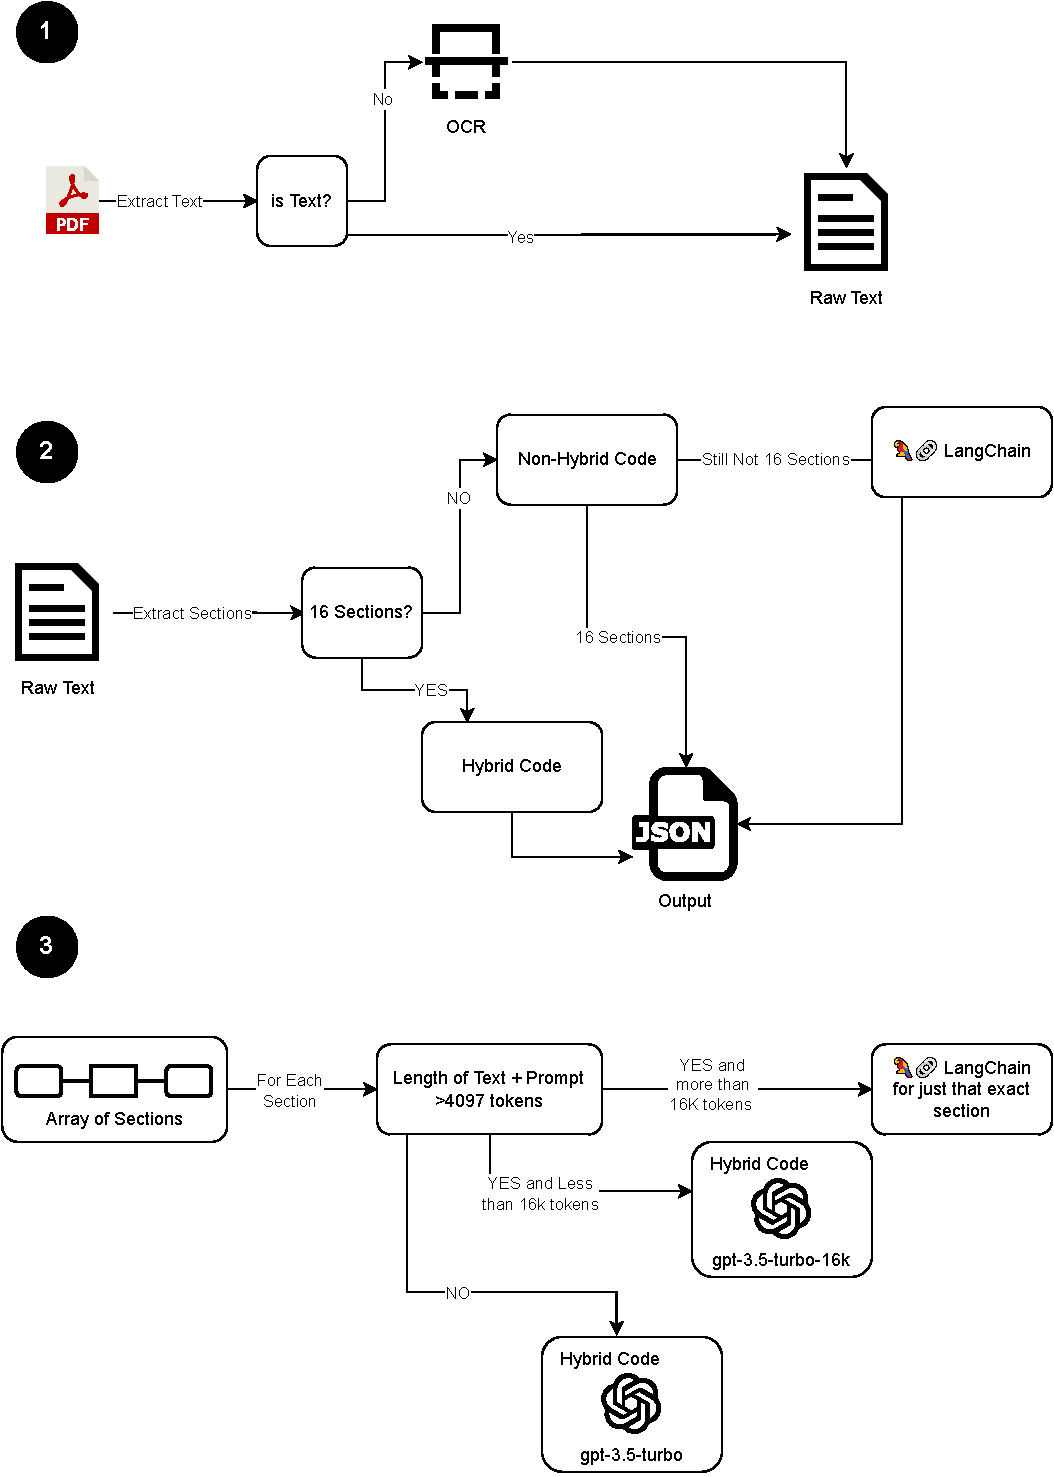
\includegraphics[width=\textwidth, keepaspectratio ]{images/bigCode}
	\caption[Improvements on Hybrid code]{Hybrid++}
\label{Hybrid++}
\end{figure}
\subsubsection{Deployment, CI pipeline}
\paragraph{Continious Integration}
As in the section on the CT prediction project, Ecomundo uses GitLab-CI, the YAML file is in \ref{appendix}. It consists of Three Stages:
\begin{enumerate}
\item \textbf{lint:} Linting is basically the automated checking of the source code for programmatic and stylistic erros. It starts by installing pyflakes since we are working with python, then runs it on the container.
\item \textbf{test:} This part of the pipeline checks whether an api or any other secret key have been left out in the code when developping or testing. Then it runs the SemGrep-SAST which stands for Semantic grep(global regex print) static application security testing. It helps by analyzing the code, finding bugs and detecting security issues.
\item \textbf{container-build:} In this stage, we are quiet sure that the code is secure and there are no problems relating to the syntax. In this case, I have already created the dockerfile, so all it has to do is build it and then push it into the docker repository of the IT team.
\end{enumerate}

\paragraph{Deployment}
The deployment comes after the docker image push into the repository. It can be done manually as well as automatically using Gitlab Helm Chart. The responsible for the creation of the helm yaml files and the deployment is Mohammed Amine ROMDHANI, the Infrastructure \& system architect.
\subsection{Results and Comments}

\section{ChatBot: EcoMundo Smart Assistant}\label{chatbot}
\subsection{Presentation of the project}

\subsection{The solution}
\subsubsection{Langchain: Context Injection}

\printglossary[title=Glossary]
\addcontentsline{toc}{chapter}{Glossary}

\bibliographystyle{plain}
\bibliography{biblio}
\addcontentsline{toc}{chapter}{Bibliography}

\appendix
\appendixpage
\addappheadtotoc
\chapter{Appendix}\label{appendix}
\begin{figure}[h]
		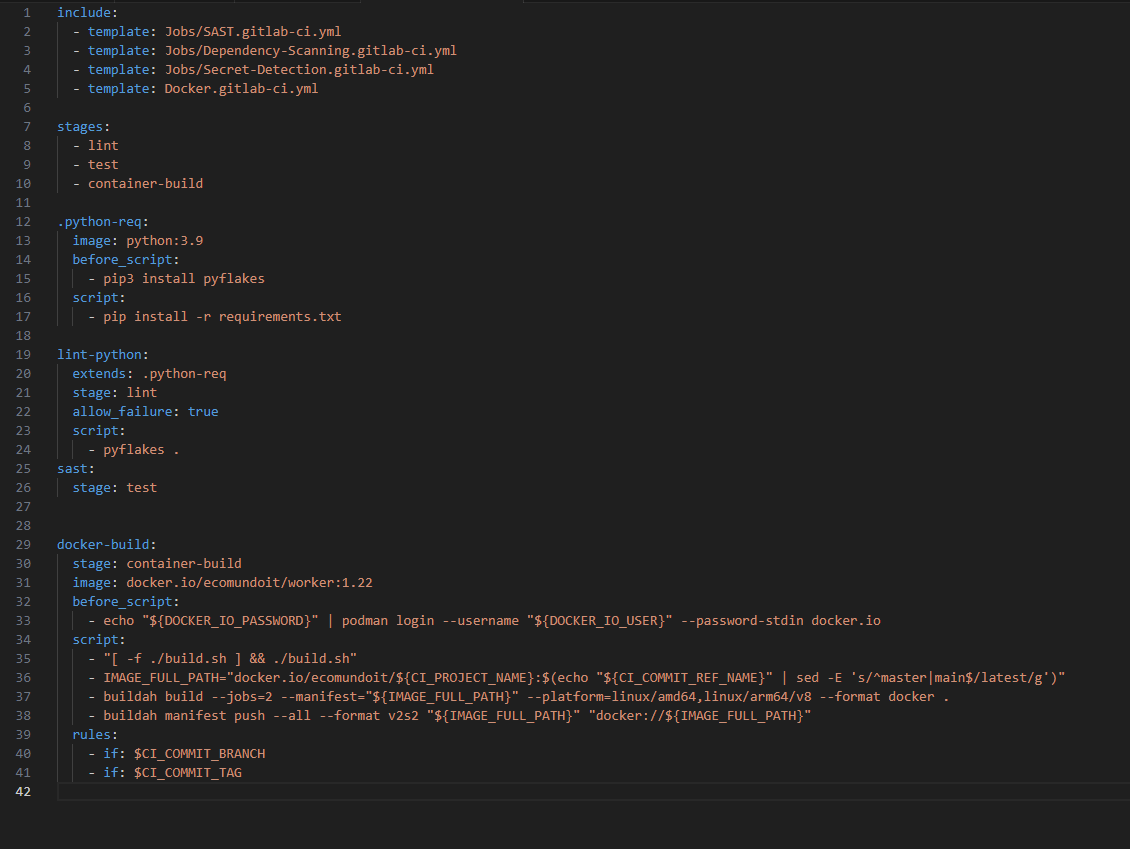
\includegraphics[width=\textwidth, keepaspectratio ]{images/python-yaml}
	\caption[Python CI pipeline]{pythonPipe}
\label{Python Pipeline}
\end{figure}
\addcontentsline{toc}{chapter}{Index}
\printindex
\newpage
\selectlanguage{french}
\begin{abstract}

\end{abstract}
\end{document}
